\section{Metodología}
\label{cap-metodo}

Para abordar la estimación de distancia a peatones desde una sola cámara RGB se diseñó una arquitectura que combina técnicas geométricas con modelado temporal, tal como se ilustra en la Fig. []. Esta arquitectura integra en un solo flujo los procesos de detección, seguimiento y análisis secuencial de características visuales, siendo capaz de operar en escenarios dinámicos desde la perspectiva de un peatón.

El núcleo del sistema consiste en identificar personas en cada ventana y construir, para cada individuo, una representación temporal basada en atributos geométricos derivados de su proyección en la imagen. Estos atributos capturan variaciones de escala y desplazamiento que reflejan de manera indirecta los cambios de distancia respecto a la cámara. Sobre estas secuencias se aplica un modelo recurrente entrenado para inferir la distancia instantánea a partir de patrones temporales.

La metodología empleada para desarrollar y validar esta arquitectura incluyó la construcción de un conjunto de datos propio mediante un modelo geométrico de referencia, la identificación y seguimiento del peatón objetivo a lo largo de cada video, la depuración y organización de las secuencias resultantes y, finalmente, el entrenamiento del modelo recurrente utilizando ventanas temporales de frames consecutivos. En las siguientes secciones se describen con detalle cada uno de estos componentes, así como su integración dentro del flujo completo de procesamiento.

\subsection{Recolección de datos}
La fase inicial consistió en la captura de secuencias de video que representen condiciones urbanas reales, grabadas con la cámara principal de un teléfono celular \textbf{Google Pixel 6 Pro} a una resolución de 1080p/30 FPS, idealmente bajo condiciones de iluminación naturales.

La cámara se sostuvo manualmente a una altura aproximada de 1.50 m en orientación horizontal, procurando mantener una posición y ángulo estables durante cada grabación. Las distancias de referencia fueron marcadas en el suelo utilizando un flexómetro, midiendo desde la posición de la cámara hasta cada punto marcado. Cada voluntario se desplazó sucesivamente hacia estas posiciones, para cada distancia marcada, el voluntario realizó desplazamientos laterales dentro de un radio acotado, manteniéndose siempre a la misma distancia aproximada de la cámara. (ver Fig. \ref{fig:diag_fija}).

\begin{figure}
    \centering
    \includegraphics[width=1\linewidth]{images/metodologia/diagrama_fija.png}
    \caption{Esquema de grabación}
    \label{fig:diag_fija}
\end{figure}

La grabación se realizó con diez voluntarios, cada uno con sus respectivas alturas (Figura \ref{fig:datos_altura}), medidas previamente a su participación; se buscó mantener alturas variadas, con el fin de evitar el sesgo de la altura más común que es de 1.70 m \cite{Velez_2025}.

\begin{figure}[H]
    \centering
    % Subfigura lateral derecho
    \begin{subfigure}{0.32\textwidth}
        \centering
        \includegraphics[width=\linewidth]{images/metodologia/tabla_alturas.png} \\
        \caption{Tabla}
        \label{subfig:table-data}
    \end{subfigure}
    \hfill
    % Subfigura central
    \begin{subfigure}{0.32\textwidth}
        \centering
        \includegraphics[width=\linewidth]{images/metodologia/histograma.png} \\
        \caption{Histograma}
        \label{subfig:histogram-heighs}
    \end{subfigure}
    \hfill
    % Subfigura lateral izquierdo
    \begin{subfigure}{0.32\textwidth}
        \centering
        \includegraphics[width=\linewidth]{images/metodologia/grafico_caja.png} \\
        \caption{Gráfico de caja}
        \label{subfig:box-heighs-persons}
    \end{subfigure}
    \caption{Alturas registradas de los voluntarios para la grabación de video, se presentan un histograma y un gráfico de caja para analizar las características de los datos}
    \label{fig:datos_altura}
\end{figure}

\subsection{Generación del conjunto de datos}
En esta etapa se procesaron las grabaciones para obtener, por cada frame relevante, el cuadro envolvente (\emph{bbox}) que delimita al sujeto de interés y las anotaciones métricas necesarias para la etapa de modelado. En el diagrama de flujo (ver Fig. \ref{fig:diag_etiquetado}) se representa de manera general el procedimiento de esta etapa.

\begin{figure}[H]
    \centering
    \includegraphics[width=\linewidth]{images/metodologia/prepro_diag.pdf}
    \caption{Pasos para etiquetar los videos y obtener anotaciones en CSV}
    \label{fig:diag_etiquetado}
\end{figure}

En primer lugar el video se subdivide en los frames correspondientes, a través de OpenCV, debido a que es importante mantener la cantidad de píxeles originales para hacer el cálculo de la distancia no se redimensiona la imagen, por lo tanto, cada frame se procesa con un tamaño de 1080x1920 píxeles, para conservar la relación entre tamaño en píxeles y distancia física del sujeto.

A continuación se pasa cada frame al procedimiento de detección y seguimiento (YOLOV8 + DeepSORT), con el objetivo de detectar a personas en el video, identificar quién de ellas es el objetivo principal, aprendiendo características del individuo en particular y realizar un seguimiento de la entidad a lo largo de toda la trayectoria que esta tomará en el transcurso de grabación. Lo anterior permite generar un \emph{bbox} de la misma persona en cada frame, y con ello las coordenadas que lo conforman.

Para evitar redundancia en el conjunto, se aplica un muestreo que elimina frames muy similares: un frame se conserva si ha transcurrido al menos 5 frames anteriormente o si por medio del cálculo de la intersección sobre la unión (IOU por sus siglas en inglés) se determina que los frames no son parecidos; cualquiera de estas dos situaciones permite que el frame siga procesándose, en caso contrario se omite y se pasa al frame siguiente.


Con la información proporcionada por el cuadro envolvente se calcula la altura de la persona en píxeles que junto con los parámetros intrínsecos de la cámara y la altura real de la persona (en milímetros) se realiza la estimación de la distancia asociada a cada frame mediante la relación física  (\ref{eq:distancia}) descrita en el trabajo mencionado en el estado del arte por \cite{wu2018sizetodepthnewperspectivesingle}.

\begin{equation}
    \text{distancia} = \frac{\text{altura}_{\text{real}}[\text{mm}] \cdot \text{distancia}_{\text{focal}}[\text{mm}] \cdot \text{tamaño}_{\text{sensor}}[\text{px}]}{\text{altura}_{\text{frame}}[\text{px}] \cdot \text{tamaño}_{\text{sensor}}[\text{mm}]}
    \label{eq:distancia}
\end{equation}

Los parámetros intrínsecos de la cámara (distancia focal y dimensiones del sensor) se obtuvieron inicialmente de las especificaciones del fabricante \cite{Google} y posteriormente se ajustaron empíricamente mediante un procedimiento de validación en campo. Para la validación se colocaron sujetos en marcas de referencia en el suelo (2.5, 5.0, 7.5, …, 25.0 m), se registraron frames representativos y se compararon las distancias calculadas mediante la ecuación (Ec. \ref{eq:distancia}) con las medidas del flexómetro. Los valores finales de los parámetros intrínsecos usados en los experimentos se recogen en la Tabla \ref{tab:intrinsec}.

\begin{table}[H]
\centering
\label{tab:intrinsec}
\begin{tabular}{lcc}
\hline
\textbf{Parámetro} & \textbf{Valor} & \textbf{Unidad} \\
\hline
Altura del sensor & 9.6 & mm \\
Resolución vertical del sensor & 1080 & píxeles \\
Distancia focal & 15 & mm \\
\hline
\end{tabular}
\caption{Parámetros intrínsecos utilizados para la estimación de distancia.}
\end{table}

 El desempeño de la relación geométrica se describe en la Tabla \ref{tab:err} y en la Figura \ref{fig:abserr}, donde se muestra la distribución del error absoluto frente a la distancia de referencia.
 
\begin{table}[H]
\centering
\label{tab:err}
\begin{tabular}{r r r r r}
\toprule
GT (m) & N muestras & Pred. mediana (m) & Error abs. (m) & Error \% \\
\midrule
2.5  & 4 & 2.8805  & 0.3805 & 15.22\% \\
5.0  & 4 & 5.0020  & 0.0020 & 0.04\% \\
7.5  & 3 & 7.4320  & 0.0680 & 0.91\% \\
10.0 & 3 & 9.9610  & 0.0390 & 0.39\% \\
12.5 & 3 & 12.2600 & 0.2400 & 1.92\% \\
15.0 & 3 & 15.2590 & 0.2590 & 1.73\% \\
17.5 & 2 & 17.4390 & 0.0610 & 0.35\% \\
20.0 & 2 & 19.7880 & 0.2120 & 1.06\% \\
22.5 & 2 & 22.4135 & 0.0865 & 0.38\% \\
25.0 & 1 & 24.5190 & 0.4810 & 1.92\% \\
\bottomrule
\end{tabular}
\caption{Resumen de la precisión por punto de referencia (mediana de las predicciones por punto).}
\end{table}

\begin{figure}[H]
    \centering
    \includegraphics[width=\linewidth]{images/metodologia/abserr.PNG}
    \caption{Dispersión del error absoluto \(|d_{\text{pred}} - d_{\text{gt}}|\) respecto a la distancia real \(d_{\text{gt}}\).}

    \label{fig:abserr}
\end{figure}

La única distancia que presenta un error significativamente mayor en el resultado es 2.5 m (\(\approx 15.22\%\)). Este efecto se debe a que a distancias muy cortas el sujeto puede no aparecer completo dentro del campo de visión de la cámara (por ejemplo, la parte superior o inferior del cuerpo queda fuera del encuadre). En ese caso el detector ajusta el \emph{bbox} al área visible y la altura en píxeles registrada para la persona queda reducida en comparación con la altura completa esperada.
Aunque el error global obtenido (\(\approx 3\%\)) incorpora todas las distancias evaluadas, este valor está condicionado por el comportamiento del modelo a 2.5 m, donde la persona no siempre aparece completamente en el encuadre y la altura del \emph{bbox} queda limitada por la propia proyección en la imagen. Este fenómeno genera una sobreestimación de la distancia y eleva el error promedio total. Para el resto del rango evaluado (que corresponde al intervalo donde la cámara capta la figura completa con mayor estabilidad) el error porcentual medio se mantiene entre 1\% y 1.2\%, lo que refleja el desempeño real del modelo en operación.

Finalmente, una vez validados los parámetros intrínsecos y obtenidas las mediciones correspondientes, se almacenaron todos los \emph{frames} etiquetados. Cada registro conserva su identificador de video y de persona, junto con las anotaciones generadas: coordenadas del cuadro envolvente, posición del punto central, altura y ancho del \emph{bbox}, así como la distancia asociada para cada instancia. Toda esta información se consolidó en un único archivo CSV que sirve como la base estructurada del conjunto de datos utilizado en el proyecto. La Figura~\ref{fig:dataDist} muestra la distribución de distancias presentes en el conjunto de datos.


\begin{figure}[H]
    \centering
    \includegraphics[width=\linewidth]{images/metodologia/annot.PNG}
    \caption{Distribución final de anotaciones por metro}
    \label{fig:dataDist}
\end{figure}


\subsection{Análisis de datos}
A partir del archivo con las anotaciones consolidadas se realizó un análisis exploratorio para justificar la selección de variables a emplear en el entrenamiento del modelo. La selección se apoyó en una matriz de correlación entre las variables anotadas y la distancia. La matriz de correlación (Figura~\ref{fig:dataCorr}) se calculó utilizando la correlación de Pearson sobre las columnas numéricas relevantes y se visualizó mediante un \emph{heatmap}.

\begin{figure}[H]
    \centering
    \includegraphics[width=\linewidth]{images/metodologia/corr.png}
    \caption{Matriz de correlación entre características geométricas y distancia}
    \label{fig:dataCorr}
\end{figure}

A partir de esta matriz se identificaron dos características con mayor correlación negativa respecto a la distancia: la altura del cuadro envolvente (bbox height, \textminus 0.84) y la coordenada vertical de su centro (y\_center, \textminus 0.30). Ambas variables se relacionan de manera inversa con la distancia real, ya que, conforme una persona se aleja de la cámara, su tamaño proyectado en la imagen disminuye y, en consecuencia, la altura del \emph{bbox} se reduce. De forma complementaria, la perspectiva de la cámara provoca que el centro del objeto se desplace gradualmente hacia la parte superior del fotograma; es decir, valores menores de y\_center suelen asociarse con objetos más lejanos.



\subsection{Análisis y Preprocesamiento de datos}

A partir del archivo con las anotaciones consolidadas se llevó a cabo un estudio detallado del conjunto de datos, orientado primero a comprender el comportamiento de las variables disponibles y posteriormente a adecuarlas para su uso en el modelo. Este proceso involucró analizar la relación entre las características geométricas y la distancia real para identificar aquellas con mayor capacidad predictiva, y, con base en ello, aplicar una serie de transformaciones destinadas a garantizar la coherencia y calidad temporal de las secuencias, homogenizar la escala de las variables y organizar la información en segmentos adecuados para su procesamiento por redes recurrentes. El flujo completo de esta etapa se resume en la Figura~\ref{fig:diag_preprocess}. Dicho esquema ilustra las ocho etapas que conforman el procedimiento, desde la depuración inicial de las anotaciones hasta la organización final de las ventanas temporales utilizadas durante el entrenamiento.

\begin{figure}[H]
    \centering
    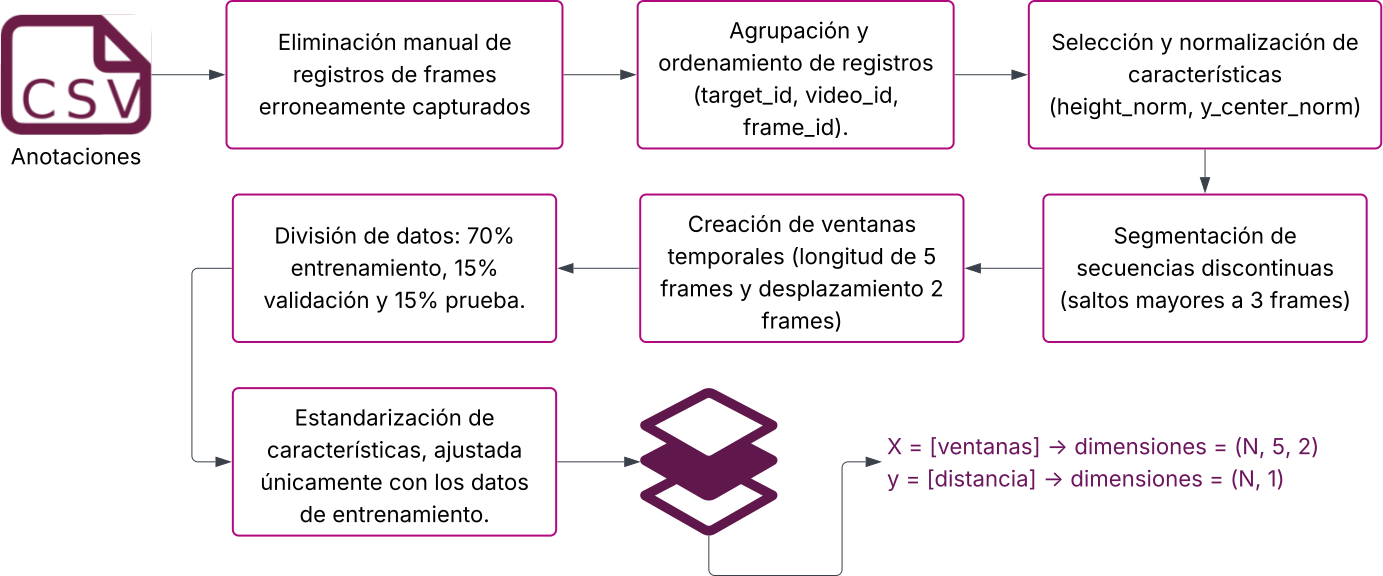
\includegraphics[width=\linewidth]{images/metodologia/preprocess_data.pdf}
    \caption{Etapas de tratamiento de las anotaciones}
    \label{fig:diag_preprocess}
\end{figure}

\subsubsection{Depuración de datos}

Durante la inspección de calidad de las anotaciones se observó que existieron errores de identificación y seguimiento provistos por el algoritmo DeepSORT (ver Fig.\ref{fig:diag_etiquetado}). Esto debido a que, ante oclusiones o cambios bruscos en la apariencia o posición, el algoritmo prioriza la asociación que minimiza su costo interno (apariencia + predicción del filtro Kalman), lo que puede conducir a confundir detecciones cercanas. Estas reasignaciones dieron lugar a distancias anotadas que no correspondían al sujeto objetivo.\\
Para detectar estos fallos se generaron versiones del video con las anotaciones (bbox, identificador de track y distancia anotada) superpuestas por cada target; esta revisión visual inicial permitió localizar y contextualizar los instantes en que las anotaciones resultaban incongruentes con la distancia conocida del sujeto.\\ 
A partir de esta referencia visual, la depuración consistió en verificar, 

\subsubsection{Análisis de datos}

A continuación, debido a la naturaleza secuencial de las redes recurrentes, se realizó la agrupación de los datos por medio del identificador de la persona y del video, esto con el fin de evitar que el modelo fuera entrenado con una secuencia que saltara de una persona a otra. 

El paso siguiente fue la selección de las características, con base en los datos proporcionados, las características relevantes tomadas fueron: la coordenada vertical del punto central del cuadro envolvente y la altura de éste recuadro. La normalización consistió en dividir dichos valores entre 1080 (altura en pixeles del frame); de tal forma que se pasa de tener las características en pixeles a tenerlas en valores de 0 a 1. 

Debido a la previa eliminación de frames con datos erróneos, la secuencia de imágenes pudo haber perdido su consistencia temporal, para corregir esto se realizaron segmentaciones; lo anterior consiste en verificar si la secuencia perdió más de 3 frames durante la limpieza de datos, y de ser así se divide la secuencia en dos diferentes, con el punto de corte justo en la posición de la pérdida de frames. Al finalizar este proceso se obtienen múltiples cadenas de frames con una correcta consistencia temporal.

Las redes neuronales recurrentes reciben secuencias de información para predecir el valor final; por lo tanto, se utiliza un tamaño de ventana que define cuántos valores va a recibir la red por cada muestra. El tamaño de ventana propuesto es de cinco valores, de cada secuencia original se tomarán esos cinco valores y se seleccionarán con un desplazamiento de dos frames hacia adelante. Además, lo anterior permite aumentar el numero de muestras, de acuerdo a la Eq.\ref{eq:n_ventanas} y mantener la dinámica temporal de la secuencia.

\begin{equation}
    N_{\text{ventanas}} = \left\lfloor \frac{L - \text{longitud\_ventana}}{\text{desplazamiento}} \right\rfloor + 1
    \label{eq:n_ventanas}
\end{equation}

Finalmente se realizó la división del conjunto de entrenamiento en un 70 porciento y 15 porciento tanto para validación como para prueba. Dentro del conjunto de entrenamiento se forzó a que los datos del individuo con la menor altura (1.51) estuvieran presentes. Con los datos de entrenamiento se ajustó la estandarización de características y se aplicaron a los demás subconjuntos.
Cada muestra tiene una dimensión de (5,2), correspondiente a 5 frames y dos características cada uno, por otro lado, el objetivo (\textit{target}) es la distancia correspondiente al último \textit{frame} en milímetros.

\subsection{Modelo de red neuronal recurrente híbrida}
\begin{figure}
    \centering
    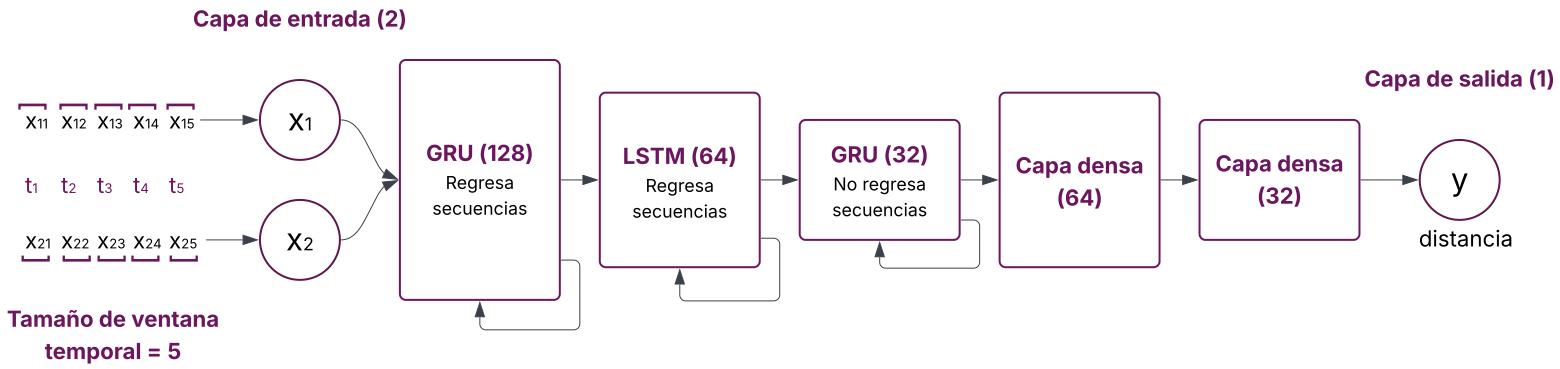
\includegraphics[width=\linewidth]{images/metodologia/nn_diagram.pdf}
    \caption{Arquitectura de la RNN híbrida}
    \label{fig:diag_nn}
\end{figure}

Debido a la naturaleza secuencial de los datos, se propone una arquitectura de red con capas de LSTM y GRU (ver Fig.\ref{fig:diag_nn}). Se tiene una entrada temporal de dos variables seguida de dos capas recurrentes y dos densas con una salida de una sola unidad. Las capas recurrentes utilizan la función de activación \texttt{tanh} para las activaciones principales y \texttt{sigmoid} para las demás, mientras que en las capas intermedias densas se utiliza \texttt{ReLU} y en la capa de salida la función \texttt{lineal}.

La función de pérdida utilizada es el error cuadrático medio (\texttt{MSE}) con el optimizador \texttt{Adam}; adicionalmente se monitorea también el error absoluto medio \texttt{MAE}. Con respecto a la regularización, se aplica \texttt{L2} de $5 \times 10^{-5}$  en las primeras dos capas recurrentes y de $1 \times 10^{-4}$ en las capas densas; se aplica \texttt{dropout} de $0.15$ para las primeras dos capas recurrentes y para las capas densas $0.25$ y $0.15$ respectivamente; también se implementaron mecanismos de regularización adaptativa mediante \texttt{EarlyStopping} y \texttt{ReduceLROnPlateau} de Keras. Las métricas de evaluación registradas son \texttt{MAE}, \texttt{MSE}, \texttt{RMSE}, \texttt{$R^{2}$}, \texttt{MAPE} y \texttt{$\sigma(AE)$}.